\subsection{Genkendelse af tegn}
\label{sec_monster}

VARIABLE!

Til genkendelse af tegn har vi arbejdet med tre forskellige metoder: Den første bruger informationer fra såkaldte \textit{middelvektorer}, den anden arbejder med såkaldte \textit{sum-billeder} mens den tredje arbejder med såkaldte \textit{forenings-billeder}. I dette afsnit vil vi beskrive disse tre metoder samt en metode til at udføre syntaksanalyse på den tegnfølge der repræsenterer nummerpladens indhold.

Metoderne til genkendelse af tegn arbejder på de syv binære billeder som separationsdelen af systemet returnerer. Metoderne returnerer syv hitlister (én for hvert billede) med tegn. Det tegn der optræder øverst på den enkelte hitliste er metodens bedste gæt på det tegn billedet forestiller, nummer to på listen er det næstbedste gæt osv. Syntaksanlysen arbejder med disse hitlister som inddata og returnerer en tegnfølge. Arbejdet der udføres i denne del af systemet er illustreret i figur \vref{fig:dia_trin3}.

\begin{figure}[htp]
\centering
\includegraphics[width=12cm]{system/illu/dia_trin3.png} 
\caption{Inddata, i form af syv billeder af tegn kommer ind i systemet fra venstre. Systemet konfigureres så en af de tre mulige metoder bruges til at genkender tegnene på billederne. Uddata er de syv tegn som en samlet tegnfølge. Da kun en af de tre metoder bruges af vores færdige system, er to af metoderne tegnet i en grå boks. Dette symboliserer at de er fravalgt.}
\label{fig:dia_trin3}
\end{figure}

Vi har udarbejdet et tegn-træningsæt bestående af tegn der er klippet ud af nummerpladerne på de 400 billeder i vores træningsæt. Vi bruger dette sæt bestående af individuelle tegn til at træne vores metoder.

%Til de tre genkendelsesmetoder har vi uarbejdet et tegn-træningssæt betående af billeder af tegn, sorteret efter tegnets type (\textbf{A}, \textbf{B}, \textbf{C} et cetera). Dette sæt er lavet ud fra vores træningssæt og vi har frasorteret billeder af tegn, hvor tegnet var afskåret. SKAL VI BESKRIVE HVORDAN DE FRAVLAGTE TEGN BLIVER SÅDAN?? Udfra dette tegn-træningssæt laver vi de enkelte træningsbilleder i de tre metoder.

\subsubsection*{Metode: Middelvektorer}
En egenskabsvektor (\textit{eng.: feature vector}) er en vektor der, som navnet antyder, repræsenterer et objekts egenskaber. I dette tilfælde er objektet et billede og egenskabsvektorerne kaldes middelvektorer. Idéen i denne metode er, at hvert billede af et tegn sammenlignes med middelvektorer (lavet på baggrund af tegn-træningssættet) for at finde det tegn som er i billedet. Der oprettes altså en middelvektor for hvert tegn. Metoden er fundet i \cite{arth}.

Først oprettes middelvektorerne. Det vil sige at der oprettes en middelvektor for tegnet \textbf{A}, tegnet \textbf{B} og så videre. Dette vektorsæt er et træningssæt (systemet "trænes" til at kende de forskellige typer af tegn). Vi definerer en middelvektor, $M$ for et antal billeder $(I_{1},I_{2},...,I_{n})$ i et træningssæt for et givent tegn således:

\begin{displaymath}
	M = (\sum_{i=1}^{n}I_i)/n
\end{displaymath}


hvor både summen og divisionen er elementvise\footnote{Ved en elementvis operation forstås at operationen udføres på alle elementer i en vektor eller matrix.}. For et testbillede af et tegn oprettes der tillige en vektor, som herefter sammenlignes med vektorerne i træningssættet for at finde den vektor der ligger nærmest billedets vektor. Tegnet for den vektor der ligger nærmest vælges.

I vores system findes afstanden, $D$ fra én middelvektor, $M = (m_{1},m_{2},...,m_{n})$ til en anden vektor, $P = (p_{1},p_{2},...,p_{n})$ i et $n$-dimensionelt rum ved brug af den euklidiske afstand\cite{wiki_euclid}:

\begin{displaymath}
	D = \sqrt{\sum_{i=1}^{n}(m_{i}-p_{i})^{2}}
\end{displaymath}

Afstande mellem to vektorer i et givent rum er illustreret i figur \vref{fig:middelvektor_afstand}.

\begin{figure}[htp]
\centering
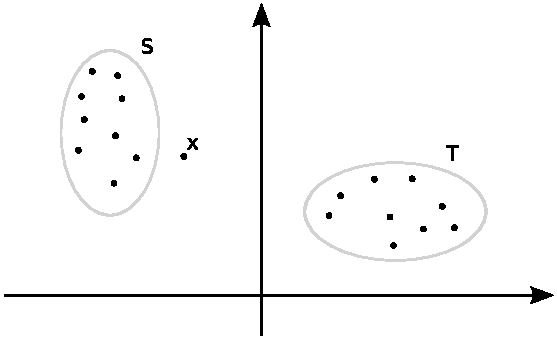
\includegraphics{system/illu/middelvektor_afstand.pdf} 
\caption{En illustration af konceptet omkring afstande mellem vektorer i et to-dimensionelt rum, hvor mængderne $S$ og $T$ angiver to træningssæt af billeder. Prikkerne i $S$ og $T$ symboliserer vektorerne for trænningsbillederne i hvert af de to sæt. $x$ er en vektor der repræsenterer et testbillede. I dette tilfælde er afstanden fra $x$ til $S$ kortere end afstanden fra $x$ til $T$, hvorfor $x$ vil blive klassificeret som det tegn der hører til $S$. I vores system arbejder vi med middelvektorer, som ville være placeret i midten af de to ellipser.}
\label{fig:middelvektor_afstand}
\end{figure}

\subsubsection*{Metode: Sum-billeder}

Denne metode ligner metoden der bruger middelvektorer. Her er idéen dog, at der oprettes såkaldte \textit{sum-billeder} for hvert tegn i stedet for middelvektorer. Metoden er lavet ud fra egen idé. HVORDAN IDEEN ER BLEVET TIL?

Hvert binære billede i træningssættet for et givent tegn skaleres til en defineret størrelse, $Z \times V$ og summeres med de andre billeder i sættet. Et eksempel på et sum-billede ses i figur \vref{fig:sumimg}.

\begin{figure}[htp]
\centering
\includegraphics[width=2cm]{system/illu/sumimg.png} 
\caption{Et eksempel på et sum-billede for tegnet \textbf{K}. De enkelte pixels intensitet angiver hvor ofte pixelen er markeret i et \textbf{K}. Jo lysere pixel, jo oftere er pixelen markeret.}
\label{fig:sumimg}
\end{figure}

Et sum-billede, $S$ konstrueres af billederne $(I_{1},I_{2},...,I_{n})$ således:

\begin{displaymath}
	S = \sum_{x=1}^n{I_x}
\end{displaymath}

hvor summen er en elementvis sum. Efter denne summering normaliseres $S$, så alle værdier i $S$ vil være mellem $0$ og $1$.
%ved at dividere alle elementer i $S$ med $\max{(S)}$. 

For hvert binære testbillede, $T$, der først skaleres til samme størrelse som $S$, multipliceres alle elementerne i $T$ med de tilsvarende elementer i $S$ og summen, $v$ tages af disse:

\begin{displaymath}
	v = \sum_{i=1}^Z{\sum_{j=1}^V{T_{ij} \cdot S_{ij}}}
\end{displaymath}

$v$ svarer altså til summen af elementer fra $S$ hvor elementet med samme koordinater i $T$ er markeret. Når $v$ er fundet for alle tegn for et testbillede, vælges tegnet hvor $v$ er maksimal.

\subsubsection*{Metode: Forenings-billeder}

I denne metode tager man alle de binære billeder i et træningssæt for et givent tegn og ser på hvilke pixels der altid er markeret i billeder af det givne tegn. Man finder altså foreningsmængden af pixels for hvert tegn. Information om denne mængde samles i noget vi har valgt at kalde forenings-billeder. Metoden er lavet ud fra egen idé.

Et forenings-billede, $F$ laves ud fra billederne $(I_{1},I_{2},...,I_{n})$ af et givent tegn som følger:

\begin{displaymath}
F = I_1 \wedge I_2 \wedge ... \wedge I_n
\end{displaymath}

hvor operatoren $\wedge$ indikerer en logisk, elementvis og-operation FORKLARING?. Et eksempel på et forenings-billede ses i figur \vref{fig:andimg}.

\begin{figure}[htp]
\centering
\includegraphics{system/illu/andimg.png} 
\caption{Et eksempel på et forenings-billede for tegnet \textbf{S}. De hvide pixels er de pixels som altid er markeret i et \textbf{S}.}
\label{fig:andimg}
\end{figure}

Når tegnet i et testbillede, $T$ skal genkendes, findes foreningsmængden af $T$ og $F$:

\begin{displaymath}
K = T \wedge F
\end{displaymath}

og antallet af markerede pixels i $K$ optælles. Det tegn, hvor antallet af markerede pixels i $K$ er maksimalt blandt alle tegnene, vælges som tegnet der repræsenteres af testbilledet.

\subsubsection*{Syntaksanalyse}

Ved syntaksanalyse analyseres tegn-hitlisterne fra de ovenstående metoder. Analysen er relevant da et gæt fra en af de to metoder måske kan udelukkes på baggrund af overtrædelse af syntaktiske regler for hele tegnfølgen. Metoden bruges i \cite{nijhuis} og \cite{kwas}.

Der kan forekomme følgende fejl i en tegnfølge fra en nummerplade i vores system:

\begin{itemize}
\item Et tal er placeret på en af de første to pladser.
\item Et bogstav er placeret på en af de sidste fem pladser.
\item Den fundne bogstavkombination er ikke tilladt\footnote{En oversigt over lovlige og ulovlige bogstavkombinationer er fundet i \cite{bogstav_komb}}.
\item Den fundne talkombination er ikke tilladt (den samlede værdi af tallene er enten for høj eller for lav)\footnote{En oversigt over tilladte talværdier er fundet i \cite{nrpl}}.
\end{itemize}

Hvis en eller flere af disse muligheder er gældende gennemser metoden hitlisterne indtil et lovligt valg af en kombination af tegn er fundet. Dette kan illustreres med følgende eksempel: Tegnfølgen \textbf{DO 45 7B3} er retuneret fra mønstergenkendelse. I denne tegnfølge forekommer der to fejl: bogstavet \textbf{O} bruges ikke på 2. position og bogstavet \textbf{B} i 6. position burde have været et tal. På 2. position itererer metoden ned igennem hitlisten til den når et bogstav som sammen med \textbf{D} danner en lovlig bostavkombination og på 6. position itereres der indtil et tal findes.

I systemet sættes en grænse for hvor langt ned ad hitlisten syntaksanalysen kan vælge tegn. Hvis denne grænse ikke fandtes, ville syntaksanalysen kunne vælge tegn som lå langt nede af hitlisten og derfor med større usikkerhed ville være det korrekte tegn.

% blot kunne itereres indtil en lovlig tegnfølge er fundet, og så ville metoderne til genkendelse af tegn give mindre mening HVIS MAN KOMMER LANGT NED I LISTERNE ER USIKKERHEDEN HØJ, DER SKAL ALTSÅ VÆLGES NOGET DER LIGNER RET MEGET. ELLER NOGET!

\subsubsection*{Metoder fra litteraturen}

I \cite{kwas} arbejder man med et simpelt, kunstigt neuralt netværk. Et kunstigt neuralt netværk er en matematisk model, som er baseret på biologiske neurale netværk\cite{wiki_nn}. I \cite{kwas} sættes antallet af neuroner i inddata-laget lig størrelsen på en matrix der repræsenterer et billede af et tegn. Antallet af neuroner i uddata-laget er lig antallet af tegn. Det neurale netværk vil derved returnerer det genkendte tegn.